\chapter*{Appendix 1: Shouty Report Processor}

The back-office team generate a report to find the most eco-friendly salesperson each month. We run a monthly contest to work out how many dollars their customers have spent on Shouty for every mile the salesperson had to travel. 

Here's how each salesperson's eco score is calculated:

\begin{verbatim}
    Eco score = Total customer revenue / Total miles travelled
\end{verbatim}

The miles travelled are taken from the sales team's monthly mileage claims spreadsheet, delivered as a CSV file.

Each row represents a trip to visit a customer. The first column is the salesperson's name. The second column is the number of miles travelled, and the third is the customer ID.

Here's an example:

\begin{verbatim}
    David Allen,13876,57
    Lisa Crispin,788,22
    Ian Dees,10383,19
    Lisa Crispin,309,137
\end{verbatim}

We use that customer ID to query the Shouty stats API, which tells us the revenue from that customer for the past 30 days.

Our batch job combines that data, calculating each salesperson's eco score to produce an XML report that will be published on the intranet.

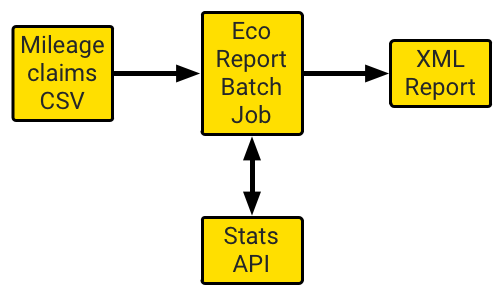
\includegraphics[width=\textwidth]{images/shouty-report-processor-overview-diagram}